\documentclass[runningheads]{llncs}

\usepackage[T1]{fontenc}
\usepackage{graphicx}
\usepackage{float}
\usepackage{booktabs}
\usepackage{cite}
\usepackage{subcaption}
\usepackage{epstopdf}

\begin{document}

\title{Pseudo-MOS Learning: A Hybrid Full-to-No-Reference FIQA Framework}

\author{André Neto\inst{1,2}\orcidID{0009-0001-0398-5859} \and % chktex 8
Nuno Gonçalves\inst{1,2}\orcidID{0000-0002-1018-4945}}
%
\authorrunning{A. Neto et al.}
% First names are abbreviated in the running head.
% If there are more than two authors, 'et al.' is used.
%
\institute{University of Coimbra \and
Institute of Systems and Robotics --- Coimbra}
%

\maketitle% typeset the header of the contribution
%
\begin{abstract}

A persistent discrepancy exists between standard Image Quality Assessment (IQA) metrics and human perceptual judgments, typically quantified through Mean Opinion Scores (MOS).
This gap poses a critical challenge for tasks where visual quality directly impacts performance, such as facial recognition and visual data transmission.
In particular, assessing the perceptual quality of steganographically distorted facial images remains difficult, especially in the absence of reference images.
To address this, we introduce a hybrid Full-to-No-Reference framework for Face Image Quality Assessment (FIQA), built upon a learning strategy based on pseudo-MOS.\@
A full-reference fusion metric is first trained by regressing multiple classical IQA scores against human MOS on a subset of a facial dataset.
This metric is then applied to the full dataset to generate pseudo-MOS labels.
Using deep features extracted from a ResNet-18 model pretrained on ImageNet, we train a no-reference regressor capable of predicting perceptual quality.
The proposed framework bridges full-reference supervision and no-reference inference, offering a scalable and accurate solution for FIQA in challenging conditions and paving the way for application-specific, data-driven IQA designs.

\keywords{Face IQA \and Steganography \and No-Reference IQA \and Pseudo-MOS \and Full-Reference Fusion \and Deep Regression}
\end{abstract}

\section{Introduction}

Image Quality Assessment (IQA) plays a critical role in domains such as biometric authentication, multimedia processing, and medical imaging~\cite{kim2015face, huang2020facerecon}. It broadly refers to the estimation of visual quality based on attributes like contrast, sharpness, noise, and the presence of artifacts. Within this domain, Facial Image Quality Assessment (FIQA) focuses specifically on facial images, where quality is not assessed in terms of visual aesthetics, but rather in terms of its impact on the performance of face recognition systems~\cite{cavazos2021racebias, terhoerst2020demobias}.

IQA methods fall into two categories: subjective and objective. Subjective methods use human ratings to measure perceived quality, often summarized as Mean Opinion Scores (MOS)~\cite{ITU-R-BT500}. These scores are reliable but expensive to collect and not scalable. Objective methods rely on algorithms to estimate quality, either by comparing to a reference image or by analyzing features of the image itself.

Objective methods can be divided into full-reference (FR) and no-reference (NR). FR methods compare a distorted image to a clean reference. They are often accurate but can only be used when a reference is available. NR methods estimate quality without a reference and are more practical in real-world settings, though they often struggle to generalize across distortions and content~\cite{shahrukh2019survey}.

FIQA is a subdomain of IQA focused on facial images. It plays a key role in biometric applications such as identity verification, where reference images are typically unavailable, and is also relevant in non-biometric scenarios like surveillance and forensic analysis. Consequently, most FIQA methods are no-reference NR, relying on task-specific priors or learned representations to estimate image quality~\cite{hernandez2019faceqnet}.

A key challenge in IQA is the gap between objective metrics and human perception. Classical metrics such as PSNR~\cite{gonzalez2002digital} (Peak Signal-to-Noise Ratio), SSIM~\cite{wang2004ssim} (Structural Similarity Index), and VIF~\cite{sheikh2006image} (Visual Information Fidelity) provide automatic quality estimates but often show weak correlation with human ratings across datasets~\cite{shahrukh2019survey}. This issue is more pronounced in facial images, where perceived quality is shaped by both image distortions and biases from the observer.

Studies have shown that FIQA is affected by both demographic and non-demographic biases. Perceived quality can vary with ethnicity, gender, or age, often due to dataset imbalance and observer subjectivity~\cite{cavazos2021racebias, terhoerst2020demobias, kabbani2024demo}. For example, darker skin tones tend to produce lower recognition accuracy, and female faces are often rated with lower quality scores~\cite{huang2020facerecon}. These effects highlight the need for more inclusive and perceptually aligned quality metrics.

The International Civil Aviation Organization~\cite{icao-2015} (ICAO) and the International Organization for Standardization (ISO) and the International Electrotechnical Commission (IEC) 19794--5 standard~\cite{iso-iec29794-5-2010} establish guidelines for image quality in Machine-Readable Travel Documents (MRTDs). These guidelines ensure uniform image conditions (e.g., lighting, focus, and resolution) and consistency across datasets. While these regulations establish a technical baseline, they do not account for perceptual biases and demographic variability in FIQA.\@

These biases raise ethical concerns. Legal frameworks, such as the European Convention on Human Rights (Article 14)~\cite{echr-article14}, the Universal Declaration of Human Rights (Article 7)~\cite{udhr-article7}, the General Data Protection Regulation (Article 22)~\cite{gdpr-article22}, the European Artificial Intelligence Act (2024)~\cite{eu-ai-act-2024} and the United States Bill of Rights~\cite{us-ai-bill-rights-2022}, aim to prevent discriminatory decisions. Still, biases persist, often introduced through human observers involved in labeling.

Neuroscience shows that face perception relies on the fusiform face area, a brain region specialized for facial stimuli~\cite{kanwisher2006fusiform, tsao2008mechanisms}. This biological specialization makes FIQA particularly sensitive to both stimulus features (e.g., age, gender, ethnicity, attractiveness) and the demographic background of the observers.

Steganographically distorted facial images pose a harder problem. Steganography hides data by slightly changing pixel values, often in ways that escape human detection~\cite{steganography}. Recent printed-proof techniques go further by ensuring that hidden data can survive physical printing and scanning noises, making them useful for secure document encoding. While these changes are visually minimal, they can damage biometric features and reduce recognition accuracy~\cite{stegastamp2020, codeface2021, stampone2024, riemannian2023}. NR methods are usually not designed to catch these small but critical degradations.

To handle these limitations, we propose a FIQA framework based on pseudo-MOS.\@ We first use a small set of facial images labeled with overall quality scores to train a fusion model that combines FR metrics into a single predictor. This model generates pseudo-MOS for the rest of the dataset. Using these labels, we then train a NR deep regressor based on a ResNet-18~\cite{resnet} pretrained on ImageNet~\cite{imagenet}, allowing it to estimate perceptual quality without needing a reference image.

Our approach bridges the gap between FR supervision and NR inference. It offers a scalable solution for evaluating images with subtle distortions, like steganography, and supports the development of quality assessment models tailored to domain-specific tasks. In doing so, it combines the accuracy of FR metrics with the practicality of NR models in a single IQA pipeline.

\section{Related Work}

To improve perceptual alignment, several fusion-based IQA methods have been proposed. Liu et al.~\cite{liu2013mmf} introduced a multi-method fusion (MMF) framework in which multiple FR-IQA scores are linearly combined through regression to better approximate human judgments. Similarly, Henniger et al.~\cite{henniger2020biosig} developed a Random Forest model trained on handcrafted image features drawn from ISO face quality standards, improving predictive utility for biometric applications. Fusion models demonstrate that integrating complementary quality cues yields superior MOS correlation compared to standalone metrics~\cite{Robinson2020}.

Beyond full-reference settings, the scarcity of ground-truth subjective scores has prompted the development of weakly supervised approaches based on pseudo-labels. Chen et al.~\cite{chen2021pseudo} proposed generating pseudo-MOS scores by averaging outputs from several FR-IQA metrics. RankIQA~\cite{liu2017rankiqa} employed synthetic degradations and relative ranking supervision to learn ordinal quality relationships. Wu et al.~\cite{wu2020cnn} used cascaded CNN regressors trained on pseudo-MOS to bootstrap NR-IQA learning. These approaches confirm the viability of pseudo-supervision in training deep IQA models when human MOS labels are limited or unavailable.

Recent progress in NR-IQA has been driven by the use of deep features from CNNs pretrained on large datasets. Kang et al.~\cite{kang2014cnn} showed that CNNs can directly regress quality scores from image patches. In the domain of FIQA, techniques such as SER-FIQ~\cite{terhorst2020serfiq} exploit the dropout-based variability of face embeddings as a proxy for image quality, while MagFace~\cite{meng2021magface} learns quality-aware facial representations by correlating embedding norms with recognition utility. QualFace~\cite{tremoco2021qualface} adapts deep face recognition models to conform with ICAO and ISO/IEC document standards, introducing an explicit quality estimation module for ID and travel document verification. These methods mark a shift from handcrafted quality indicators to learned feature-level representations tailored to face recognition tasks.


Other studies emphasize that image quality is inherently task-specific. In FIQA, quality is defined not by visual aesthetics but by its impact on face recognition performance. Standards such as ISO/IEC 19794--5 codify this operational perspective, specifying conditions for acceptable biometric image acquisition. Supervised models like FaceQnet~\cite{hernandez2019faceqnet} learn to predict face utility scores directly from embeddings. Datasets such as PIPAL~\cite{jin2020pipal}, which include generative distortions, further highlight the need for context-specific IQA evaluation. Our work follows this trajectory by targeting steganographically degraded facial images, an emerging use case not addressed in current FIQA literature.

\section{Methodology}\label{sec:methodology}

\subsection{Dataset}

For practical reasons we decided to use the publically available Face Research Lab London (FRLL) Set~\cite{DeBruine2017}, an ICAO compliant dataset that consists of 102 neutral frontal facial images alongside metadata on attractiveness provided by over 2500 observers. We carefully selected 15 demographically diverse facial
images out of the dataset, shown in Fig.~\ref{fig:subdataset}. Each image was subsequently processed using four printer-proof steganography methods, each applied at nine encoding threshold levels. This approach introduced a diverse range of quality distortions, yielding a total of 555 images, including their original references.

\begin{figure}[!htbp]
    \centering
    \includegraphics[width=1\linewidth]{images/subdataset.png}
    \caption{Sample images from the FRLL dataset.}\label{fig:subdataset}
\end{figure}

The used printer-proof steganography methods are based on Generative Adversarial Networks (GANs)~\cite{gans2018} to encode and decode information, we can obtain various results depending on the method used:

\begin{itemize}
    \item StegaStamp~\cite{stegastamp2020}: claims to be the first steganography model capable of decoding data from printed images. The authors show robust results in decoding data under physical transmission by developing novel strategies to add noise in the training process, printer noise simulation, and distortion for the training dataset.
    \item CodeFace~\cite{codeface2021}: encoder and decoder networks are trained using end-to-end GANs. It introduces a new security system for encoding and decoding facial images that are printed in common IDs and MRTDs.
    \item RiemStega~\cite{cruz2025riemstega}: proposes a new loss function that extends the loss function based on the $L_2$ distance between images to the Riemannian manifold of symmetric and positive definite matrices.
    \item StampOne~\cite{stampone2023}: focuses on high-level robust steganography, such as~\cite{codeface2021, stegastamp2020}, striking a balance between high-quality encoded images and decoding accuracy. It mitigates distortion-related issues like JPEG compression, camera sensors and printer's Gaussian noise by incorporating gradient transform, wavelet transform, and Depthwise~\cite{tay2022efficient} to normalize and balance frequencies of the inputs. 
\end{itemize}

Each image in our dataset was evaluated approximately 30 times by human observers, providing a robust Mean Opinion Score (MOS) dataset.

We followed ITU-R BT.500 --- 15~\cite{ITU-R-BT500} recommendation, and adopted the Single Stimulus method. Around 200 different observers were carefully instructed on how to perform the test session, the average duration of the session was 22 minutes, and the average number of tests in each session was 70. Resulting in over 14,000 images being evaluated.

To conduct the sessions we created a webapp, seen in Fig.~\ref{fig:platform}, where the observers conceded their demographic data (age, gender, ethnicity, etc.) and were asked to evaluate each image on a scale from 1 to 100 using a slider bar, for as long as they wanted. The rating scale was divided into five categorical levels: scores from 1 to 25 were classified as Bad, 26 to 50 as Poor, 51 to 75 as Fair, 76 to 99 as Good, and a score of 100 as Excellent.

\begin{figure}[!htbp]
    \centering
    \includegraphics[width=0.7\linewidth]{images/webapp.png}
    \caption{Custom webapp platform used to access overall image quality.}\label{fig:platform}
\end{figure}

We collected observer's demographic (age, gender, ethnicity, and country of origin) and non-demographic information (education level, device being used, and place where test was being performed).

\subsection{Statistical Bias Analysis}

Considering that the homogeneity of variances assumption is not met, we performed Welch's analysis of variance (ANOVA) to examine the impact of observer demographics --- gender (140 male, 60 female), ethnicity (173 causasian, 8 latino, 8 black, and others), and age grouped into categories (under 18, 18 --- 25, 26 --- 40, 41 --- 60, over 60) as well as subject demographic and non-demographic (attractiveness) characteristics on MOS.\@ The statistical significance of each factor was evaluated using a threshold of $p < 0.01$, and effect size analysis was conducted using Eta Squared~\cite{cohen1988statistical} ($\eta^2$) to quantify the relative contribution of each variable.

\subsubsection{Impact of Observer Demographics on MOS}

According to table~\ref{tab:anova_observer}, ethnicity, gender and age significantly impact MOS scores, suggesting that subjective evaluations of image quality are influenced by observer characteristics. Post-hoc Tukey's HSD~\cite{tukey1949comparing} tests were conducted to determine specific group differences, identifying notable discrepancies across demographic subgroups. The presence of these biases underscores the need for IQA methodologies that incorporate perceptual fairness considerations.


\begin{table}[!htbp]
\caption{Welch's ANOVA results for observer demographics.}
\begin{center}
\begin{tabular}{|l|c|c|c|c|}
\hline
\textbf{Factor} & \textbf{Welch F} & \textbf{DF} & \textbf{p-value} & \textbf{Eta Squared}  \\
\hline
Observer Gender & 6.97 & 1 & 0.00112 & 0.012 \\ \hline
Observer Ethnicity & 9.36 & 8 & 5.65e-13 & 0.027 \\ \hline
Observer Age Group & 33.00 & 4 & $\cong$ 0 & 0.045 \\ \hline
\end{tabular}\label{tab:anova_observer}
\end{center}
\end{table}

\subsubsection{Impact of Image Characteristics on MOS}

Table~\ref{tab:anova_image} presents the influence of subject demographic and non-demographic characteristics on MOS.\@ Results suggest that MOS is influenced by aesthetic preferences and other visual factors, reinforcing its inherently subjective nature.

\begin{table}[!htbp]
\caption{Welch's ANOVA results for subject characteristics.}
\begin{center}
\begin{tabular}{|l|c|c|c|c|}
\hline
\textbf{Factor} & \textbf{Welch F} & \textbf{DF} & \textbf{p-value} & \textbf{Eta Squared} \\
\hline
Subject Gender & 19.84 & 1 & 5.87e-06 & 0.018 \\
\hline
Subject Ethnicity & 8.85 & 3 & 7.38e-06 & 0.022 \\
\hline
Subject Age Group & 11.62 & 4 & 4.82e-35 & 0.033 \\
\hline
Attractiveness & 18.04 & 1 & 2.18e-05 & 0.015 \\
\hline
\end{tabular}\label{tab:anova_image}
\end{center}
\end{table}

\subsubsection{Observer-Subject Interaction Effects on MOS}

A two-way ANOVA was performed to analyze the interaction effects between observer demographics and subject characteristics.

\begin{table}[!htbp]
\centering
\caption{Two-way ANOVA interaction effects.}
\begin{tabular}{|l|c|c|c|c|} \hline
\textbf{Observer $\times$ Subject} & \textbf{F-value} & \textbf{DF} & \textbf{p-value} & \textbf{Eta Squared} \\ \hline
Gender & 2.31 & 1 & 0.0654 & 0.006 \\ \hline
Ethnicity & 1.51 & 24 & 0.0556 & 0.011 \\ \hline
Age Group & 2.87 & 16 & 1.94e-10 & 0.024 \\ \hline
\end{tabular}\label{tab:anova_interaction}
\end{table}

These findings confirm the existence of demographic bias in MOS ratings, making it crucial to account for such biases when using subjective scores in image quality assessment models. The effect size analysis using Eta Squared ($\eta^2$) provides insight into the relative contribution of each factor to MOS variance. Our results reinforce the need for better FIQA models to correct demographic biases.

\subsection{Image Quality Metrics}

A total of 41 different Image Quality Assessment (IQA) metrics were evaluated, spanning traditional signal-based measures (e.g., PSNR, SSIM), perceptual-based metrics (e.g., FSIM, VIF), and deep-learning-based approaches (e.g., LPIPS, DISTS). The correlation between these metrics and MOS was analyzed using Pearson’s and Spearman’s correlation coefficients. 

Fig.~\ref{fig:mos_vs_iqa} presents scatter plots comparing MOS values against individual IQA metrics. Each plot illustrates the relationship between subjective evaluations and objective IQA scores, highlighting the varying degrees of correlation among metrics. Some metrics, such as FSIM and MS-SSIM~\cite{wang2003multiscale}, demonstrate a strong monotonic relationship with MOS.\@ These visualizations justify the need for a fusion-based approach to optimize MOS predictability.


\begin{figure}[h]
    \centering
    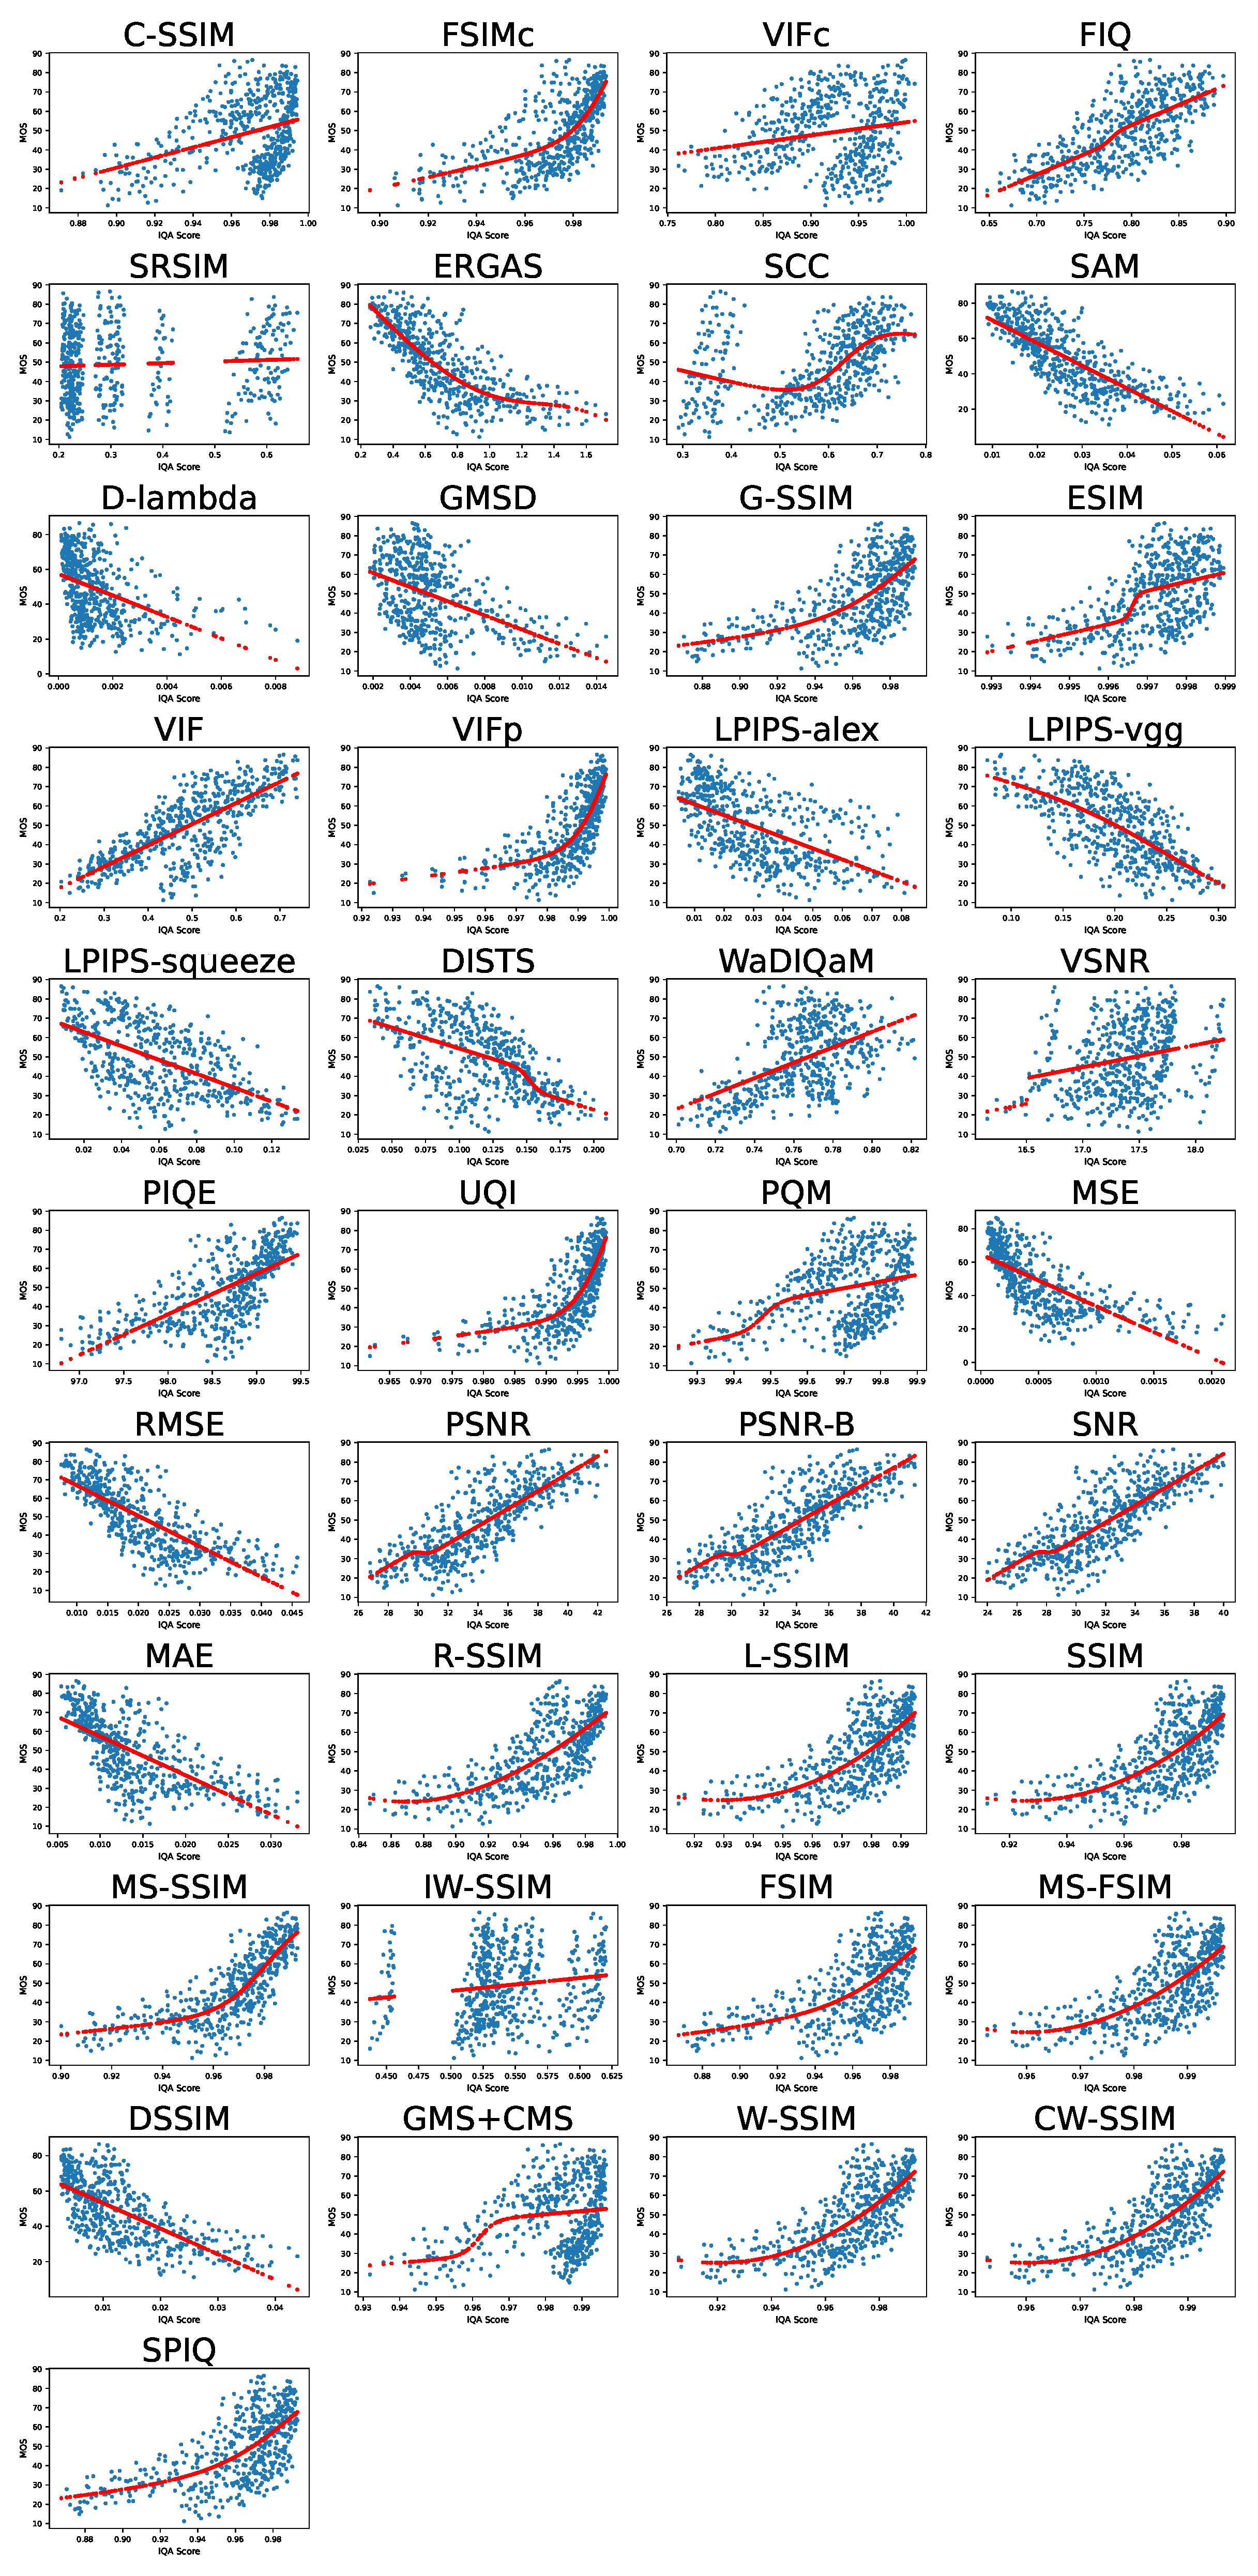
\includegraphics[width=\linewidth]{images/mos_vs_iqa_grid.eps}
    \caption{Scatter plots illustrating the relationship between Mean Opinion Scores (MOS) and individual Image Quality Assessment (IQA) metrics.}\label{fig:mos_vs_iqa}
\end{figure}

\subsection{Fusion-Based Image Quality Assessment}

To improve the correlation between IQA metrics and MOS, we implemented a fusion-based approach integrating multiple quality measures. The fusion process involved weighting individual IQA metrics based on their predictive performance relative to MOS.\@ We explored several fusion techniques, including:

\begin{itemize}
    \item Principal Component Analysis (PCA): Used to reduce redundancy among IQA metrics and derive an optimized linear combination.
    \item Regression-Based Models: Linear regression and ridge regression were applied to determine the best combination of metrics that predict MOS effectively.
    \item Machine Learning Approaches: A Random Forest~\cite{breiman2001random} (RF) model was trained using individual IQA metrics as input features, leveraging nonlinear interactions to improve MOS correlation. The dataset was split into 80\% for training and 20\% for testing. The model was configured with 100 trees (\textit{n\_estimators = 100}) and used the MSE criterion for optimization.

\end{itemize}

To assess the effectiveness of individual and fusion-based IQA metrics, we employed two correlation measures:

\begin{itemize}
    \item Pearson's Linear Correlation Coefficient (PLCC): Evaluates the linear relationship between IQA scores and MOS.\@
    \item Spearman's Rank-Order Correlation Coefficient (SRCC): Measures the monotonic relationship between IQA scores and MOS, accounting for nonlinearity in observer perception.
\end{itemize}

\subsection{Implementation Details}

The experiments were conducted using Python. The dataset went through a post-screening process to normalize IQA scores and eliminate outliers. Training and evaluation followed a five-fold cross-validation strategy to ensure robust model performance.

\section{Results}

\subsection{Ranking of Individual IQA Metrics}

The correlation analysis between individual IQA metrics and MOS revealed significant variability in their predictive performance. Fig.~\ref{fig:ranking} presents a ranked comparison of the 41 evaluated IQA metrics based on the arithmetic mean of the Pearson and Spearman correlation coefficients. Metrics such as MS-SSIM, SAM, and PSNR-B~\cite{ma2011psnr} demonstrated the highest correlation with MOS, suggesting that these metrics consistently align with subjective perception of distortions in facial images.

\begin{figure}[htbp]
    \centering
    \includegraphics[width=\linewidth]{images/fusion_metric_ranking.eps}
    \caption{Ranking of IQA Metrics Based on Fusion Metric (PLCC \& SRCC).}\label{fig:ranking}
\end{figure}

\subsection{Comparison of Fusion Models}

To evaluate the effectiveness of different fusion techniques, we compared multiple approaches, including PCA-based fusion, ridge regression, and random forest-based models. Fig.~\ref{fig:fusion_vs_mos} summarizes the performance of these models in terms of PLCC and SRCC, indicating that the random forest fusion method yielded the highest correlation with MOS.\@

The results indicate that machine learning-based fusion techniques outperform statistical fusion approaches such as PCA and regression. The random forest fusion model effectively captures nonlinear interactions between IQA metrics, enabling more accurate predictions of subjective image quality. PCA, while useful for dimensionality reduction, discards some potentially valuable information, leading to lower correlation coefficients. Regression-based models, constrained by their linear nature, also fall short in capturing complex dependencies among IQA metrics.

\begin{figure}[htbp]
    \centering
    \includegraphics[width=\linewidth]{images/fusion_model_vs_mos.png}
    \caption{Scatter plot of Fusion-Based IQA Scores vs. MOS.}\label{fig:fusion_vs_mos}
\end{figure}

\subsection{Correlation Between Fusion Scores and MOS}

The application of fusion models significantly improved the correlation between IQA scores and MOS.\@ Fig.~\ref{fig:final_comparison_grid} illustrates the relationship between the optimized fusion scores and MOS values, demonstrating a substantial improvement in correlation coefficients.
While deep learning models could further enhance performance, the Open Source Face Image Quality (OFIQ) framework prioritizes simple and fast implementations, making it the most suitable choice for this study.

These results underscore the advantage of integrating multiple IQA metrics to obtain a more reliable predictor of MOS.\@ The success of the fusion model suggests that no single IQA metric is sufficiently comprehensive to capture the full range of perceptual quality factors, but rather, a combination of complementary metrics provides the most robust estimation.

Overall, the findings highlight the superiority of machine learning-based fusion strategies in FIQA.\@ The improved MOS predictability achieved through fusion further supports the hypothesis that integrating multiple complementary metrics enhances the robustness of IQA systems. Additionally, these results provide insights into the design of more accurate quality assessment models that align better with human perception.

\begin{figure}[htbp]
    \centering
    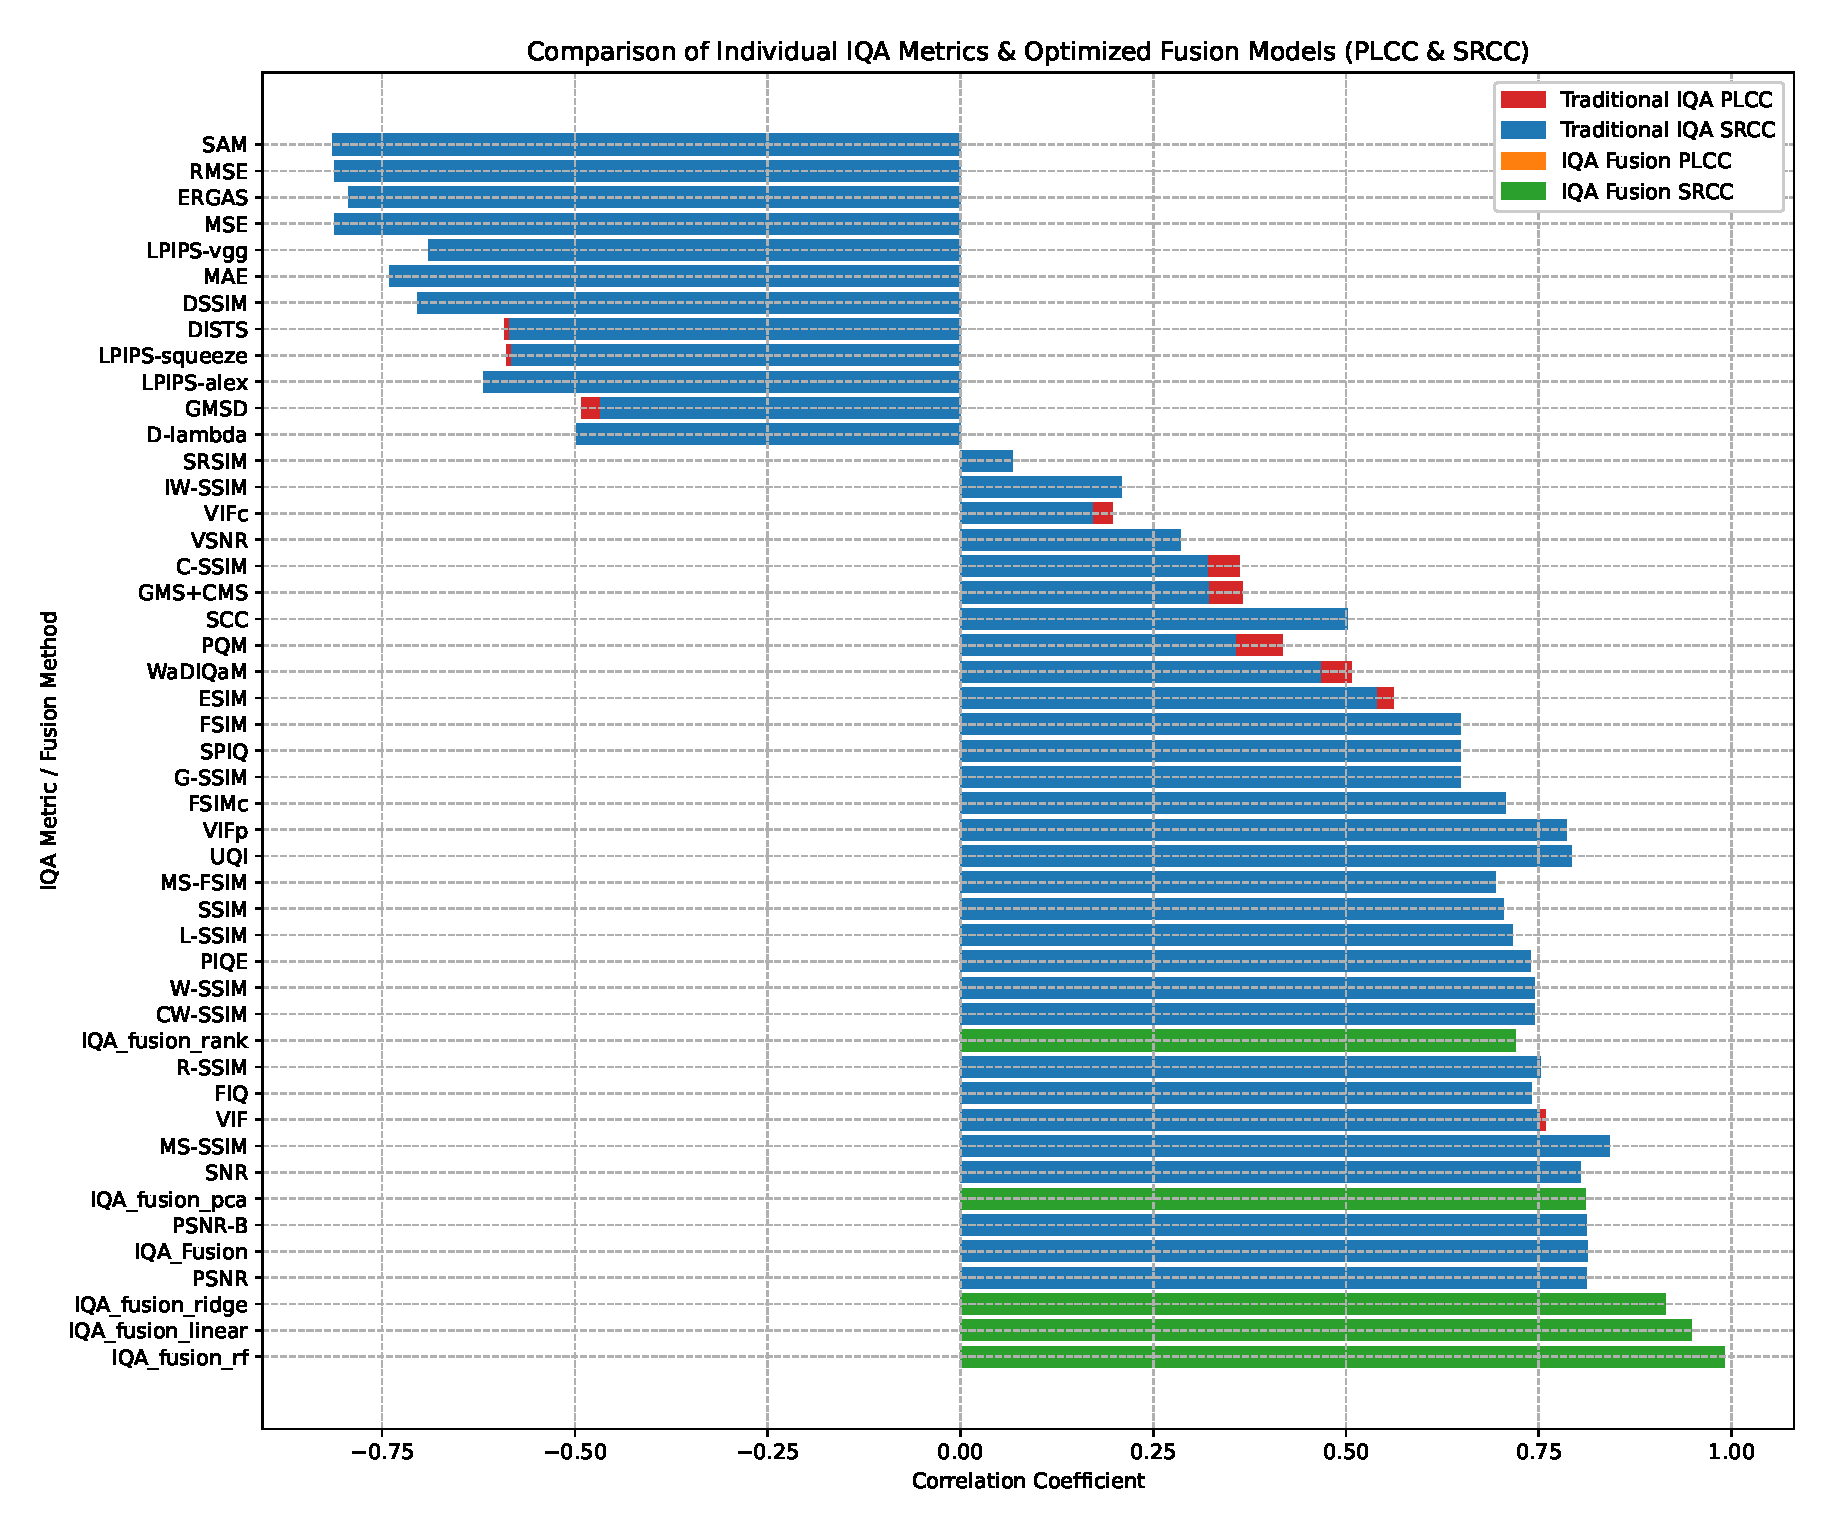
\includegraphics[width=\linewidth]{images/iqa_vs_fusion_iqa.eps}
    \caption{Comparison of IQA metrics and Optimized Fusion Models (PLCC \& SRCC)}\label{fig:final_comparison_grid}
\end{figure}
\section{Conclusion and Future Work}

We proposed a Full-to-No-Reference framework for FIQA that predicts image quality in the absence of reference images by leveraging a pseudo-MOS supervision strategy. Our method first trains a FR fusion model to regress human perceptual judgments on a labeled subset (10\% of the dataset), generating pseudo-MOS labels for a larger unlabeled dataset. These forged labels are then used to train a deep NR regressor, enabling quality prediction from distorted images alone. This two-stage pipeline effectively bridges the gap between fully supervised FR-IQA and reference-free NR-IQA approaches.

Beyond the development of our NR IQA metric, the proposed framework offers a flexible foundation for constructing a variety of task-specific models. By enabling scalable, perceptually grounded supervision with limited ground-truth annotations, our approach can facilitate quality-aware training in applications such as GANs, forensic imaging, and domain-adapted biometric pipelines.

\section{Acknowledgments}

The author would like to thank Dr.\ Shahrukh Athar for his support during the initial state-of-the-art review. His comprehensive list of implemented IQA metrics from his work were invaluable in kick-starting this study.
The author also gratefully acknowledges the Institute of Systems and Robotics (ISR) for providing the resources and research environment that made this work possible.
Lastly, we gratefully acknowledge everyone who contributed to the MOS labeling process, as their efforts were crucial in establishing the foundation for our research.
This study has received funding from the EU Horizon Europe for the  ACHILLES project under Grant Agreement No. 101189689, and FCT -- Fundação para a Ciência e a Tecnologia, I.P., under the project UIDB/00048/2020 (DOI 10.54499/UIDB/00048/2020). % chktex 8

\bibliographystyle{ieeetr}
\bibliography{references}

\end{document}
